%% bare_conf.tex
%% V1.4b
%% 2015/08/26
%% by Michael Shell
%% See:
%% http://www.michaelshell.org/
%% for current contact information.
%%
%% This is a skeleton file demonstrating the use of IEEEtran.cls
%% (requires IEEEtran.cls version 1.8b or later) with an IEEE
%% conference paper.
%%
%% Support sites:
%% http://www.michaelshell.org/tex/ieeetran/
%% http://www.ctan.org/pkg/ieeetran
%% and
%% http://www.ieee.org/

%%*************************************************************************
%% Legal Notice:
%% This code is offered as-is without any warranty either expressed or
%% implied; without even the implied warranty of MERCHANTABILITY or
%% FITNESS FOR A PARTICULAR PURPOSE! 
%% User assumes all risk.
%% In no event shall the IEEE or any contributor to this code be liable for
%% any damages or losses, including, but not limited to, incidental,
%% consequential, or any other damages, resulting from the use or misuse
%% of any information contained here.
%%
%% All comments are the opinions of their respective authors and are not
%% necessarily endorsed by the IEEE.
%%
%% This work is distributed under the LaTeX Project Public License (LPPL)
%% ( http://www.latex-project.org/ ) version 1.3, and may be freely used,
%% distributed and modified. A copy of the LPPL, version 1.3, is included
%% in the base LaTeX documentation of all distributions of LaTeX released
%% 2003/12/01 or later.
%% Retain all contribution notices and credits.
%% ** Modified files should be clearly indicated as such, including  **
%% ** renaming them and changing author support contact information. **
%%*************************************************************************


% *** Authors should verify (and, if needed, correct) their LaTeX system  ***
% *** with the testflow diagnostic prior to trusting their LaTeX platform ***
% *** with production work. The IEEE's font choices and paper sizes can   ***
% *** trigger bugs that do not appear when using other class files.       ***                          ***
% The testflow support page is at:
% http://www.michaelshell.org/tex/testflow/


\label{beginning of document}
\documentclass[conference]{IEEEtran}
% Some Computer Society conferences also require the compsoc mode option,
% but others use the standard conference format.
%
% If IEEEtran.cls has not been installed into the LaTeX system files,
% manually specify the path to it like:
% \documentclass[conference]{../sty/IEEEtran}

\usepackage{graphicx}
	\graphicspath{{images/}} 
\renewcommand\IEEEkeywordsname{Keywords}
\usepackage{hyperref}
	\hypersetup{colorlinks=true,allcolors=blue}
\usepackage{hypcap}
\usepackage{listings}
	\lstset{
  		frame=single,
  		basicstyle=\ttfamily\scriptsize,
  		breaklines=true
	}
\usepackage{subfig}

% Some very useful LaTeX packages include:
% (uncomment the ones you want to load)


% *** MISC UTILITY PACKAGES ***
%
%\usepackage{ifpdf}
% Heiko Oberdiek's ifpdf.sty is very useful if you need conditional
% compilation based on whether the output is pdf or dvi.
% usage:
% \ifpdf
%   % pdf code
% \else
%   % dvi code
% \fi
% The latest version of ifpdf.sty can be obtained from:
% http://www.ctan.org/pkg/ifpdf
% Also, note that IEEEtran.cls V1.7 and later provides a builtin
% \ifCLASSINFOpdf conditional that works the same way.
% When switching from latex to pdflatex and vice-versa, the compiler may
% have to be run twice to clear warning/error messages.






% *** CITATION PACKAGES ***
%
%\usepackage{cite}
% cite.sty was written by Donald Arseneau
% V1.6 and later of IEEEtran pre-defines the format of the cite.sty package
% \cite{} output to follow that of the IEEE. Loading the cite package will
% result in citation numbers being automatically sorted and properly
% "compressed/ranged". e.g., [1], [9], [2], [7], [5], [6] without using
% cite.sty will become [1], [2], [5]--[7], [9] using cite.sty. cite.sty's
% \cite will automatically add leading space, if needed. Use cite.sty's
% noadjust option (cite.sty V3.8 and later) if you want to turn this off
% such as if a citation ever needs to be enclosed in parenthesis.
% cite.sty is already installed on most LaTeX systems. Be sure and use
% version 5.0 (2009-03-20) and later if using hyperref.sty.
% The latest version can be obtained at:
% http://www.ctan.org/pkg/cite
% The documentation is contained in the cite.sty file itself.






% *** GRAPHICS RELATED PACKAGES ***
%
\ifCLASSINFOpdf
  % \usepackage[pdftex]{graphicx}
  % declare the path(s) where your graphic files are
  % \graphicspath{{../pdf/}{../jpeg/}}
  % and their extensions so you won't have to specify these with
  % every instance of \includegraphics
  % \DeclareGraphicsExtensions{.pdf,.jpeg,.png}
\else
  % or other class option (dvipsone, dvipdf, if not using dvips). graphicx
  % will default to the driver specified in the system graphics.cfg if no
  % driver is specified.
  % \usepackage[dvips]{graphicx}
  % declare the path(s) where your graphic files are
  % \graphicspath{{../eps/}}
  % and their extensions so you won't have to specify these with
  % every instance of \includegraphics
  % \DeclareGraphicsExtensions{.eps}
\fi
% graphicx was written by David Carlisle and Sebastian Rahtz. It is
% required if you want graphics, photos, etc. graphicx.sty is already
% installed on most LaTeX systems. The latest version and documentation
% can be obtained at: 
% http://www.ctan.org/pkg/graphicx
% Another good source of documentation is "Using Imported Graphics in
% LaTeX2e" by Keith Reckdahl which can be found at:
% http://www.ctan.org/pkg/epslatex
%
% latex, and pdflatex in dvi mode, support graphics in encapsulated
% postscript (.eps) format. pdflatex in pdf mode supports graphics
% in .pdf, .jpeg, .png and .mps (metapost) formats. Users should ensure
% that all non-photo figures use a vector format (.eps, .pdf, .mps) and
% not a bitmapped formats (.jpeg, .png). The IEEE frowns on bitmapped formats
% which can result in "jaggedy"/blurry rendering of lines and letters as
% well as large increases in file sizes.
%
% You can find documentation about the pdfTeX application at:
% http://www.tug.org/applications/pdftex





% *** MATH PACKAGES ***
%
%\usepackage{amsmath}
% A popular package from the American Mathematical Society that provides
% many useful and powerful commands for dealing with mathematics.
%
% Note that the amsmath package sets \interdisplaylinepenalty to 10000
% thus preventing page breaks from occurring within multiline equations. Use:
%\interdisplaylinepenalty=2500
% after loading amsmath to restore such page breaks as IEEEtran.cls normally
% does. amsmath.sty is already installed on most LaTeX systems. The latest
% version and documentation can be obtained at:
% http://www.ctan.org/pkg/amsmath





% *** SPECIALIZED LIST PACKAGES ***
%
%\usepackage{algorithmic}
% algorithmic.sty was written by Peter Williams and Rogerio Brito.
% This package provides an algorithmic environment fo describing algorithms.
% You can use the algorithmic environment in-text or within a figure
% environment to provide for a floating algorithm. Do NOT use the algorithm
% floating environment provided by algorithm.sty (by the same authors) or
% algorithm2e.sty (by Christophe Fiorio) as the IEEE does not use dedicated
% algorithm float types and packages that provide these will not provide
% correct IEEE style captions. The latest version and documentation of
% algorithmic.sty can be obtained at:
% http://www.ctan.org/pkg/algorithms
% Also of interest may be the (relatively newer and more customizable)
% algorithmicx.sty package by Szasz Janos:
% http://www.ctan.org/pkg/algorithmicx




% *** ALIGNMENT PACKAGES ***
%
%\usepackage{array}
% Frank Mittelbach's and David Carlisle's array.sty patches and improves
% the standard LaTeX2e array and tabular environments to provide better
% appearance and additional user controls. As the default LaTeX2e table
% generation code is lacking to the point of almost being broken with
% respect to the quality of the end results, all users are strongly
% advised to use an enhanced (at the very least that provided by array.sty)
% set of table tools. array.sty is already installed on most systems. The
% latest version and documentation can be obtained at:
% http://www.ctan.org/pkg/array


% IEEEtran contains the IEEEeqnarray family of commands that can be used to
% generate multiline equations as well as matrices, tables, etc., of high
% quality.




% *** SUBFIGURE PACKAGES ***
%\ifCLASSOPTIONcompsoc
%  \usepackage[caption=false,font=normalsize,labelfont=sf,textfont=sf]{subfig}
%\else
%  \usepackage[caption=false,font=footnotesize]{subfig}
%\fi
% subfig.sty, written by Steven Douglas Cochran, is the modern replacement
% for subfigure.sty, the latter of which is no longer maintained and is
% incompatible with some LaTeX packages including fixltx2e. However,
% subfig.sty requires and automatically loads Axel Sommerfeldt's caption.sty
% which will override IEEEtran.cls' handling of captions and this will result
% in non-IEEE style figure/table captions. To prevent this problem, be sure
% and invoke subfig.sty's "caption=false" package option (available since
% subfig.sty version 1.3, 2005/06/28) as this is will preserve IEEEtran.cls
% handling of captions.
% Note that the Computer Society format requires a larger sans serif font
% than the serif footnote size font used in traditional IEEE formatting
% and thus the need to invoke different subfig.sty package options depending
% on whether compsoc mode has been enabled.
%
% The latest version and documentation of subfig.sty can be obtained at:
% http://www.ctan.org/pkg/subfig




% *** FLOAT PACKAGES ***
%
%\usepackage{fixltx2e}
% fixltx2e, the successor to the earlier fix2col.sty, was written by
% Frank Mittelbach and David Carlisle. This package corrects a few problems
% in the LaTeX2e kernel, the most notable of which is that in current
% LaTeX2e releases, the ordering of single and double column floats is not
% guaranteed to be preserved. Thus, an unpatched LaTeX2e can allow a
% single column figure to be placed prior to an earlier double column
% figure.
% Be aware that LaTeX2e kernels dated 2015 and later have fixltx2e.sty's
% corrections already built into the system in which case a warning will
% be issued if an attempt is made to load fixltx2e.sty as it is no longer
% needed.
% The latest version and documentation can be found at:
% http://www.ctan.org/pkg/fixltx2e


%\usepackage{stfloats}
% stfloats.sty was written by Sigitas Tolusis. This package gives LaTeX2e
% the ability to do double column floats at the bottom of the page as well
% as the top. (e.g., "\begin{figure*}[!b]" is not normally possible in
% LaTeX2e). It also provides a command:
%\fnbelowfloat
% to enable the placement of footnotes below bottom floats (the standard
% LaTeX2e kernel puts them above bottom floats). This is an invasive package
% which rewrites many portions of the LaTeX2e float routines. It may not work
% with other packages that modify the LaTeX2e float routines. The latest
% version and documentation can be obtained at:
% http://www.ctan.org/pkg/stfloats
% Do not use the stfloats baselinefloat ability as the IEEE does not allow
% \baselineskip to stretch. Authors submitting work to the IEEE should note
% that the IEEE rarely uses double column equations and that authors should try
% to avoid such use. Do not be tempted to use the cuted.sty or midfloat.sty
% packages (also by Sigitas Tolusis) as the IEEE does not format its papers in
% such ways.
% Do not attempt to use stfloats with fixltx2e as they are incompatible.
% Instead, use Morten Hogholm'a dblfloatfix which combines the features
% of both fixltx2e and stfloats:
%
% \usepackage{dblfloatfix}
% The latest version can be found at:
% http://www.ctan.org/pkg/dblfloatfix




% *** PDF, URL AND HYPERLINK PACKAGES ***
%
%\usepackage{url}
% url.sty was written by Donald Arseneau. It provides better support for
% handling and breaking URLs. url.sty is already installed on most LaTeX
% systems. The latest version and documentation can be obtained at:
% http://www.ctan.org/pkg/url
% Basically, \url{my_url_here}.




% *** Do not adjust lengths that control margins, column widths, etc. ***
% *** Do not use packages that alter fonts (such as pslatex).         ***
% There should be no need to do such things with IEEEtran.cls V1.6 and later.
% (Unless specifically asked to do so by the journal or conference you plan
% to submit to, of course. )


% correct bad hyphenation here
\hyphenation{op-tical net-works semi-conduc-tor}


\begin{document}
%
% paper title
% Titles are generally capitalized except for words such as a, an, and, as,
% at, but, by, for, in, nor, of, on, or, the, to and up, which are usually
% not capitalized unless they are the first or last word of the title.
% Linebreaks \\ can be used within to get better formatting as desired.
% Do not put math or special symbols in the title.
\title{Towards Model-Driven\\Gamified Software Modelling Learning}


% author names and affiliations
% use a multiple column layout for up to three different
% affiliations
\author{\IEEEauthorblockN{Alfa Yohannis\IEEEauthorrefmark{1}, Dimitris Kolovos, Fiona Polack}
\IEEEauthorblockA{Department of Computer Science\\
University of York\\
York, United Kingdom\\
Email: \IEEEauthorrefmark{1}ary506@york.ac.uk}}

% conference papers do not typically use \thanks and this command
% is locked out in conference mode. If really needed, such as for
% the acknowledgment of grants, issue a \IEEEoverridecommandlockouts
% after \documentclass

% for over three affiliations, or if they all won't fit within the width
% of the page, use this alternative format:
% 
%\author{\IEEEauthorblockN{Michael Shell\IEEEauthorrefmark{1},
%Homer Simpson\IEEEauthorrefmark{2},
%James Kirk\IEEEauthorrefmark{3}, 
%Montgomery Scott\IEEEauthorrefmark{3} and
%Eldon Tyrell\IEEEauthorrefmark{4}}
%\IEEEauthorblockA{\IEEEauthorrefmark{1}School of Electrical and Computer Engineering\\
%Georgia Institute of Technology,
%Atlanta, Georgia 30332--0250\\ Email: see http://www.michaelshell.org/contact.html}
%\IEEEauthorblockA{\IEEEauthorrefmark{2}Twentieth Century Fox, Springfield, USA\\
%Email: homer@thesimpsons.com}
%\IEEEauthorblockA{\IEEEauthorrefmark{3}Starfleet Academy, San Francisco, California 96678-2391\\
%Telephone: (800) 555--1212, Fax: (888) 555--1212}
%\IEEEauthorblockA{\IEEEauthorrefmark{4}Tyrell Inc., 123 Replicant Street, Los Angeles, California 90210--4321}}




% use for special paper notices
%\IEEEspecialpapernotice{(Invited Paper)}




% make the title area
\maketitle

% As a general rule, do not put math, special symbols or citations
% in the abstract
\begin{abstract}
\label{abstract}
Backgrounded by the challenges in teaching and learning software modelling, this research harnesses the engaging nature of games, the effectiveness of pedagogy, and the automation of Model-driven Engineering to propose a platform for model-driven gamified software modelling learning. It is an environment for tutors where they can create new and make use of existing software modelling learning activities for teaching and for learners to learn software modelling topics in a gameful way. This paper presents the rationale of the idea behind the initiation of the platform as well as its design considerations which mostly are withdrawn from game, pedagogy, and model-driven domains. An introduction to the concept of substate is statechart modelling demonstrated to show how the platform works, and some identified significant challenges and open issues are also discussed as important lessons for further research and development.
\end{abstract}

% no keywords
\begin{IEEEkeywords} 
model-driven, gameful, software modelling, learning, platform
\end{IEEEkeywords}



% For peer review papers, you can put extra information on the cover
% page as needed:
% \ifCLASSOPTIONpeerreview
% \begin{center} \bfseries EDICS Category: 3-BBND \end{center}
% \fi
%
% For peerreview papers, this IEEEtran command inserts a page break and
% creates the second title. It will be ignored for other modes.
\IEEEpeerreviewmaketitle



\section{Introduction}

\section{Rationale}
Software modelling teaching and learning (SMTL) has significant role in model-driven domain, since it establishes the very foundation in Model-driven Engineering (MDE) learners whom in the future will be MDE experts and practitioners. If the process of SMTL can be improved, it will bring benefits not just to learners but also to model-driven domain and wider related domains. So, what are the challenges in SMTL? How they should be addressed? 

The first challenge is the abstraction. It is the very nature attribute of modelling since modelling is the process of thinking abstractly about systems \cite{bezivin2009teaching}. Some writers emphasise the cruciality of abstraction in computer science and software engineering \cite{Kramer2007, hazzan2008reflections, Saitta2013} in general as well as model-driven domain  \cite{engels2005teaching, borstler2012teaching, whittle2013industrial, brambilla2012model} in particular. 

The nature of abstraction makes the concepts being learned are difficult to access since the concepts are only accessible through tangible representation, such as symbols and diagrams \cite{Duval2006}. Even though the abstract concepts have visualized, engagement can still be an issue, that is making learners to actively participate in learning processes. This is the condition where gameful approach comes into play to solve motivational issues. Game elements can be embedded into learning activities to present gameful experience.  

Other problem is to posses abstraction skills--ability to perform abstractive operations, such as selecting the appropriate abstraction level, moving through different abstraction levels, and view abstraction from different perspectives. To learn the abstraction skills,  Some experts suggest that teaching and learning abstraction should start from familiarizing with real-world objects an then move upwards to abstraction through similarity \cite{engels2005teaching,white2010teaching}. However, the process of abstraction could continue to move downwards to reification and then finally to application\cite{white2010teaching}. Hazzan suggests that in order to grasp abstract concepts, they should be experienced--seen, felt, and used. Therefore, the concepts should be illustrated, reflected, and practised by learners \cite{hazzan2008reflections}. Supporting tutors to perform these approaches will help them tackling the abstraction challenge. 
  
The second challenge is the contents of SMTL. Some experts suggest the contents should be definitions, semantics, syntaxes, notations of modelling \cite{Borstler2012}, other experts point the core concepts of MDE--modelling, metamodelling, and model transformation--and their applications \cite{bezivin2009teaching}, and others prompt the engineering aspect of software modelling should not be neglected \cite{paige2014bad}. While main ideas of the contents have been proposed by experts, the detail structures how the contents should be organised is not clear yet. For example, statechart modelling has concepts of states, transitions, decisions, regions, and etc. There might be some structures that are best these concepts for teaching and learning statechart modelling and it is good to follow such structures. However, there are no 'one-for-all' structures that fit to all contexts, creativity of tutors, and learners. So rather than only following the best structures, it is best to support tutors to express organisation of the contents based on their preferences and needs, regardless whether they are inspired by the best structures or not.

The third challenge is the teaching and learning Approaches. One approach in to teach software modelling broadly, throughout, and not deeply\cite{Borstler2012, paige2014bad}, so they learn to decide which modelling process is more appropriate than others \cite{Akayama2013}. Other approach is harnessing modelling tools which are very important to tackle large-scale modelling and ecourage to produce good models \cite{Akayama2013}. However, failure to provide enough supports (e.g. helpful instructions and expert tools) might overwhelm learners with unnecessary features \cite{liebel2015ready}. These are just two Approaches of many other Approaches proposed by experts in software modelling. On the other side, the field of pedagogy also have employed collections of approaches for teaching and learning in general, for examples, Bloom's taxonomy \cite{krathwohl2002revision}, Kolb's experiential learning \cite{kolb2014experiential}, and Keller's ARCS motivational model \cite{keller2010motivational}. All of these approaches are worth to be considered in SMTL and should not be neglected. However, considering the same reason that applies to contents there are no 'one-for-all' approaches, it is best to support tutors to design their own approaches in SMTL, whether they follows the existing approaches or their own creativity.   

On the other side, MDE provides a convenient way to produce software \cite{stahl2006model}. The software itself could act as a platform for tutors to create 
contents and approaches for teaching certain concepts in software modelling in the form of 
learning activities and also for learners to engage with the learning activities. MDE offers the advantages to speed up the development of the learning activities. First, using the platform, tutors can harness a high-level visual modelling language to design the learning activities at high-level abstraction. Second, the platform automates the generation of runnable instances of the learning activity design, which with the runnable instances learners can perform software modelling learning.

To sum up, in order to improve SMTL, two conditions have to be met. First, SMTL should be engaging for learners. This could be done through embedding game elements into learning activities. Second, SMTL should be creative. Tutors are given supports to create new and reuse existing SMTL contents and approaches, whether inspired by existing good practices or just according to their own creativity. Thus, to satisfy these conditions, a platform for model-driven gamified software modelling learning is proposed. It is an environment for tutors where they can create new and make use of existing software modelling learning activities for teaching and for learners to learn software modelling topics in a gameful way.

Once the platform can be fully utilised, it will empower tutors to express their creativity in producing different patterns of learning activities, whether the learning activities are based on existing best practices or new approaches in teaching certain concepts in SMTL. The platform will also ease learners in learning software modelling since the learning activities are presented a gameful way. As soon as many learning activities are available, the learners can choose learning patterns that is best for them and exercise through many different patterns. 

All interaction of tutors and learners with the platform can be logged and logs are the source of data which further could be used to extract knowledge to understand deeper about  teaching and learning behaviours in software modelling. Using analytical techniques, such as machine learning and data mining, questions like which part or learning activity that learners often make mistakes, what parts of software modelling that are most challenging for them, what strategies that they prefer to use to construct models for certain problems, and many other questions could be answered and understood. The understanding that could change the way software modelling is taught and learned. Moreover, the platform could also be a place for research and experiment. For example, comparing two learning patterns which one is better in teaching one same concept in software modelling and  investigating which shapes that are more appropriate to represent a certain concept in a visual modelling language. With further development, the platform could also support 'multiplayers' which means collaboration in SMTL could also be supported. This also means concepts like collaborative learning and content creation can also be tested and applied into SMTL. 



\section{Design}

\subsection{Gameful Design}
\subsection{Pedagogical Design}
\subsection{Model-Driven Design}



\section{Demonstration}
In this section, an example is presented to demonstrate the use of the platform. The example is to show the of teaching the concept of substates in UML statechart modelling. In this demonstration, designers are assumed to have proficient knowledge and skills of statechart diagram while learners are assumed already understood the concept of states, transitions, start state, and final state. The following subsections are the order of the statechart from its definition to be fully used in a game play.
 
\subsection{Define Statechart Metamodel}
In order for the platform to support modelling in statechart diagram, designers have to define its metamodel first. The metamodel is written in Emfatic (\url{https://www.eclipse.org/emfatic}) and Eugenia-like annotations \cite{kolovos2015eugenia} are used to define its concrete syntax. For example, the definition of Start State derived from Node class is displayed in Fig. \ref{metamodel}. Other basic elements of statechart diagram, such as states, transitions, end states, etc., are also defined but not displayed in the figure.  

\begin{figure}[th]
\centering
\begin{lstlisting}
abstract class Node extends Entity {
  ref Edge[*]#source outgoing;
  ref Edge[*]#target incoming;
}

@node(label="name", dhape="startState", whiteSpace="wrap", html="1", fillColor="#000000", width="30", height="30")
class Start extends Node {
}
\end{lstlisting} 
\caption{A definition of Start State derived from Node class using Emfatic and Eugenia-like annotations.}
\label{metamodel}
\end{figure}

The annotated metamodel then trasformed using Epsilon \cite{kolovos2010epsilon} and EMF (\url{http://www.eclipse.org/modeling/emf/}) to generate the Java codes of the metamodel, as the backbone codes for further model operations, and Javascript codes to display the statechart's elements as visual elements in a palette of an MxGraph-based graphical editor (\url{https://jgraph.github.io/mxgraph/}). 

\subsection{Create Statechart Model}
Using the MxGraph-based graphical editor (Fig. \ref{ide}), designers can now create statechart models. The editor has a pallete on the left side that contains elements of statechart's elements which they can drag and drop into a drawing area on the centre where they can arrange the elements to construct statechart models. The editor also has a property panel on the right side to modify the attributes and appearance of the models. Models that have been created can be saved and loaded again for further operations. The editor also can be used to create models as input/base models to be embedded in learning activities.        

\begin{figure}[th]
\centering
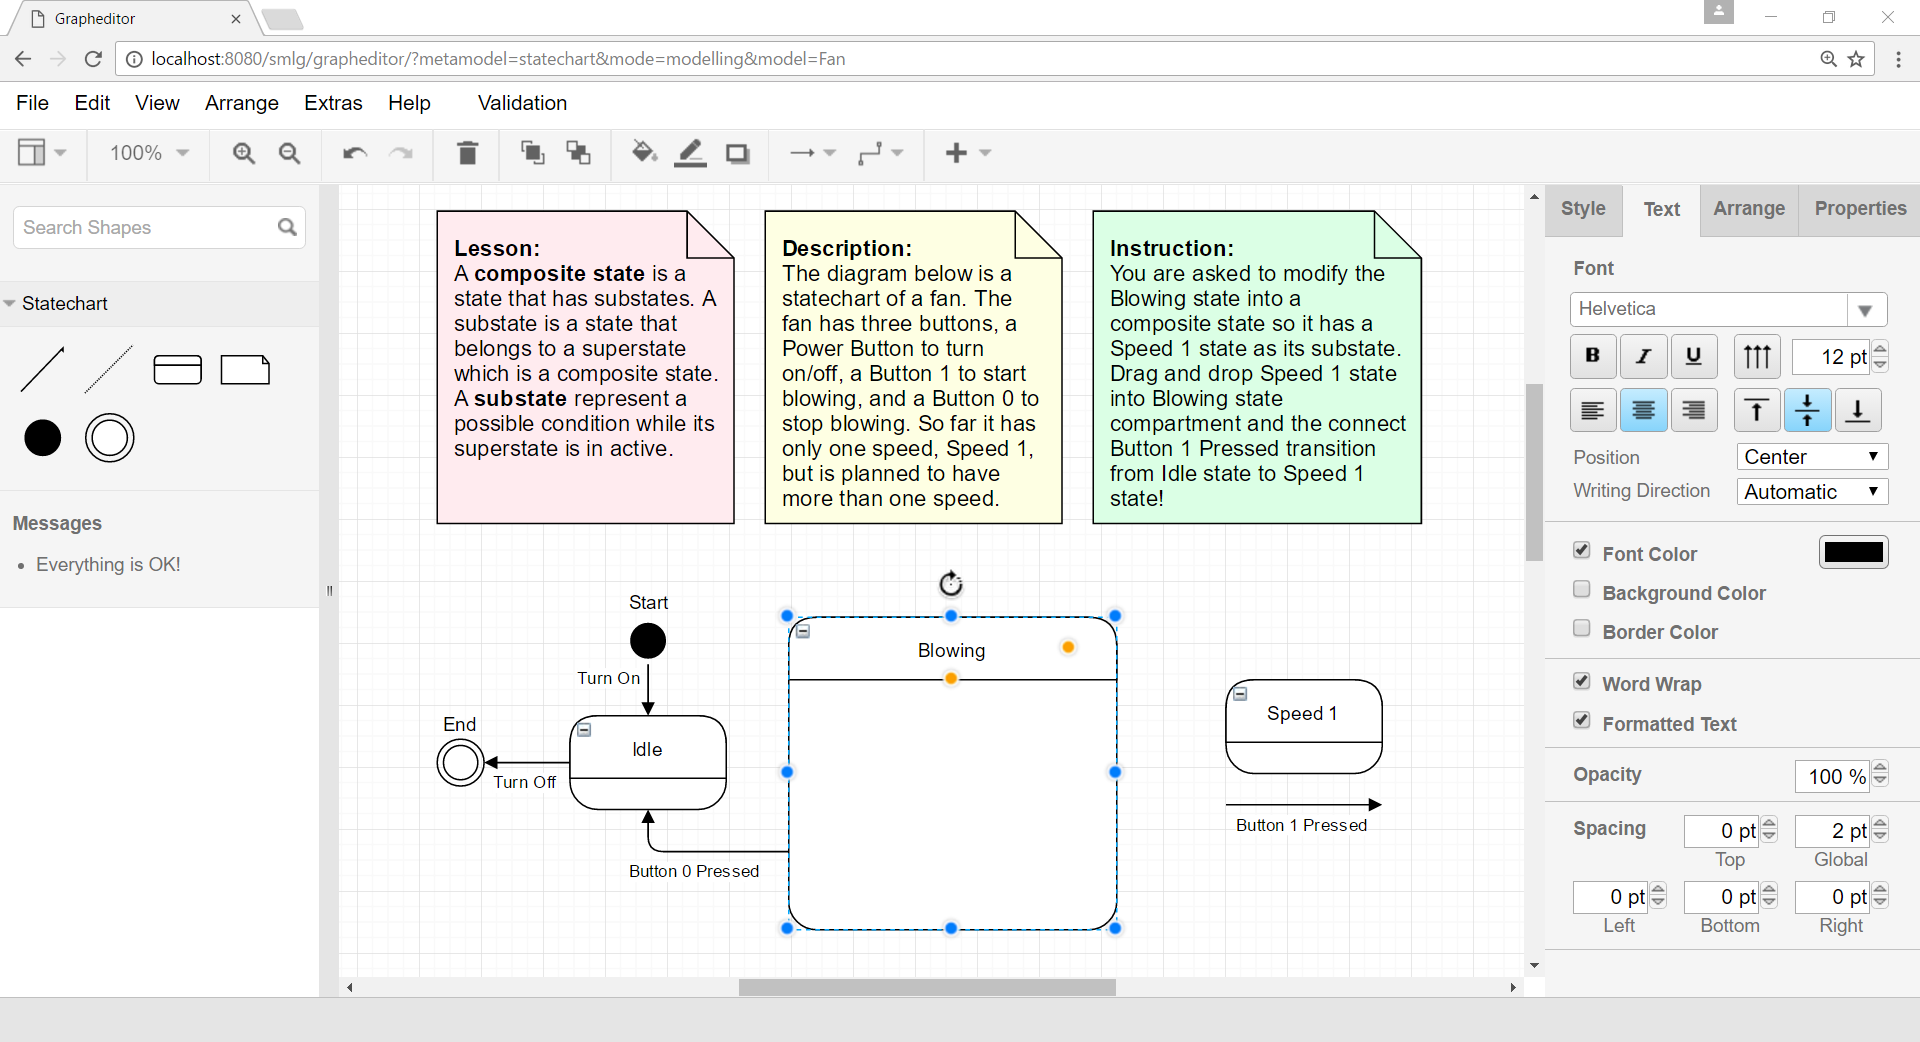
\includegraphics[width=\linewidth]{ide}
\caption{The MxGraph-based graphical editor to create statechart models.}
\label{ide}
\end{figure}

\subsection{Create Learning Pattern Model}
To teach and learn a concept, designers have to design a learning pattern that consists of ordered learning activities. In this example, a learning pattern to learn the concept of substates is created (Fig. \ref{eoml}). The case that is selected is an electrical fan that has two main states, Idle and Blowing. Learners will be asked to modify the Blowing state so it becomes composite state that has several substates that represent different speed of blowing. The learning pattern has three activities, namely One-Speed Fan, Two-Speed Fan, and Tree-Speed Fan. The activities are arranged \textit{per se} to accommodate Flow state \cite{csikszentmihalyi2014toward} so learners can start learning from the easiest activity to the hardest one. The activities are explained in more detail  in the next following subsections.
  
\begin{figure}[th]
\centering
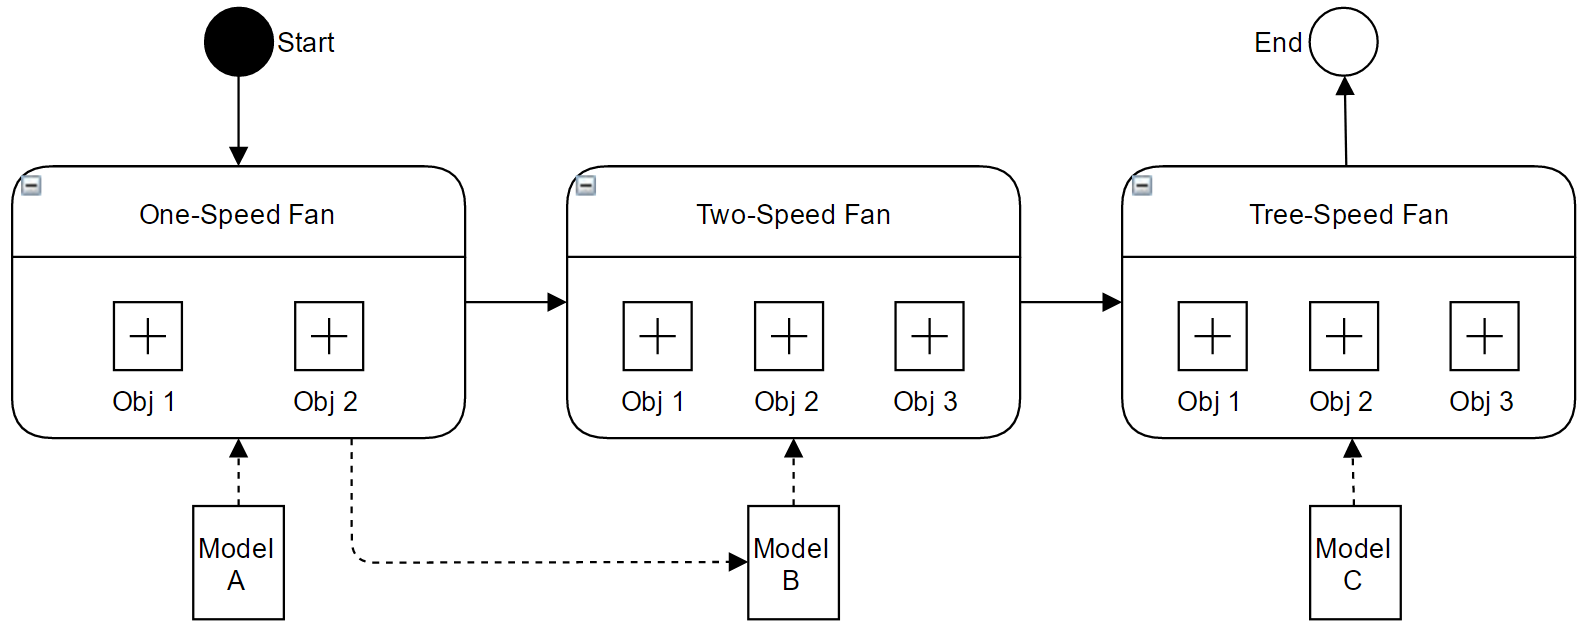
\includegraphics[width=\linewidth]{eoml}
\caption{A learning activity pattern for learning the concept of Substates in state-machine modelling.}
\label{eoml}
\end{figure}

Each activity has lesson and instruction properties. Lesson contains explanation about the concepts that are being taught and instruction contains commands or questions that learners need to execute or answer. In the process of satisfying the instruction in each activity, one or more objectives have to be met by learners in order to move to next activity. Also, each activity can consume existing models (Model A, B, and C in Fig. \ref{eoml}) as its base models so learners do not have to create a model from scratch and produce model (Model B in Fig. \ref{eoml}) to be used in its next activity. Each of the models also has a description property to describe itself which is very useful for learners to understand about the model. An example of the lesson, model description, and instruction properties of the One-Speed Fan activity (Fig. \ref{eoml}) is displayed in Fig. \ref{example-01a}.    

\begin{figure}[th]
\centering
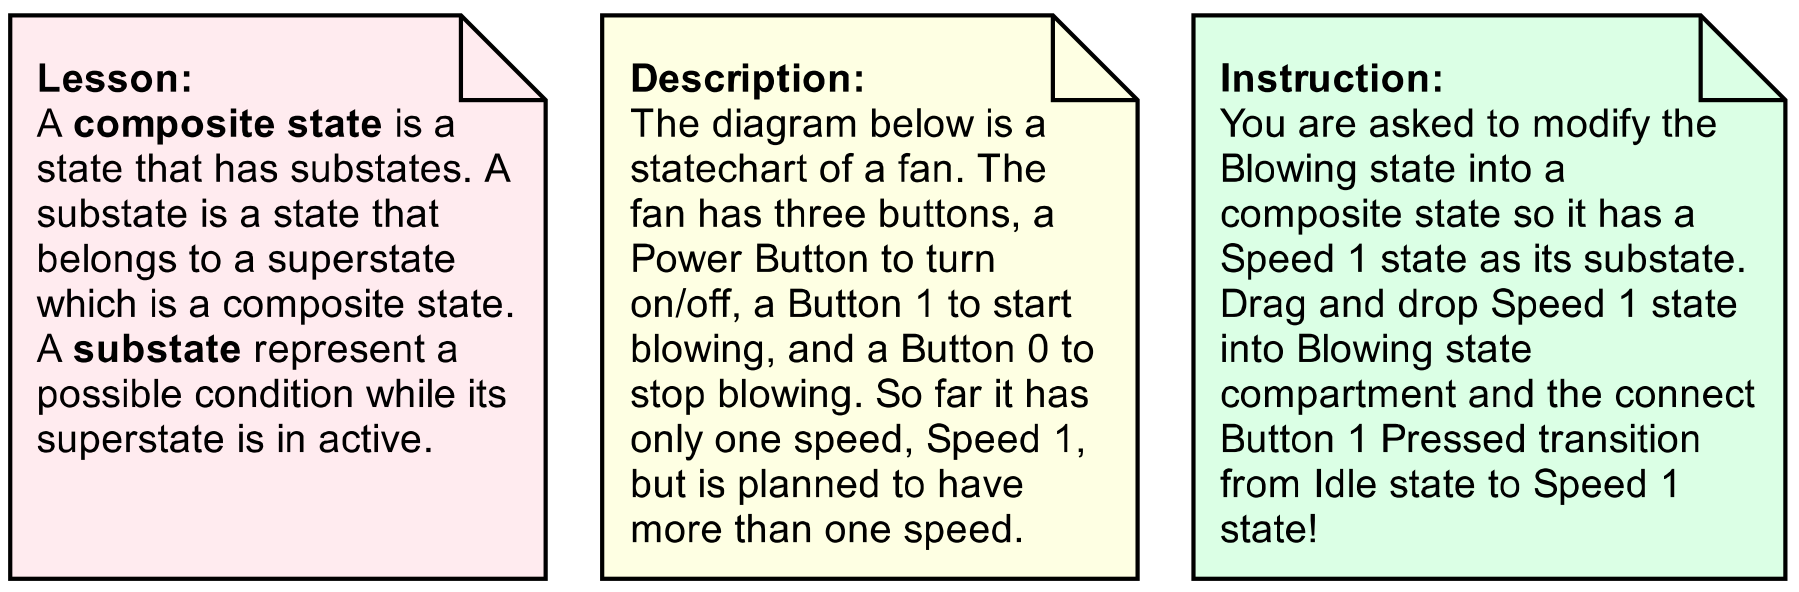
\includegraphics[width=\linewidth]{example-01a}
\caption{Lesson, model description, and instruction.}
\label{example-01a}
\end{figure}

\subsubsection{One-Speed Fan Activity}
In this activity (Fig. \ref{example-01}), learners are introduced to one substate only.The activity start with a base model and learners are required to modify the base model (Fig. \ref{example-01b}) to meet the target model (Fig. \ref{example-01c}). The base model corresponds to Model A in Fig. \ref{eoml}, which refers to an existing model that already created previously and will be loaded once the activity is executed so leaners do not need to create the model from the start. 

The example case in this activity is a fan that has three buttons, a Power Button to turn on/off, a Button 1 to start blowing, and a Button 0 to stop blowing. So far it has only one speed, Speed 1, but is planned to have more than one speed. Learners are asked to modify the Blowing state in Fig. \ref{example-01b} into a composite state through moving the Speed 1 state into the Blowing state compartment as well as to connect the Button 1 Pressed transition from the Idle state to the Speed 1 state. Since in Fig. \ref{eoml} this activity is designed to have only two objectives, the two objectives are adjusted and defined as follow: Objective 1 "Blowing state contains Speed 1 substate" and Objective 2 "Button 1 Pressed transition connects Idle state to Speed 1 substate".

\begin{figure}[th]
    \centering
    \subfloat[Base model]{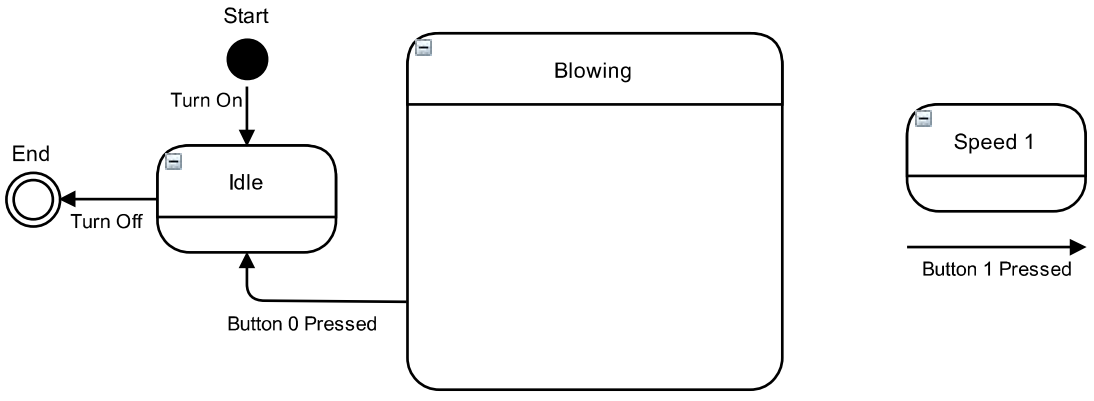
\includegraphics[width=\linewidth]{example-01b}	
    \label{example-01b}}
    \\
    \subfloat[Target model]{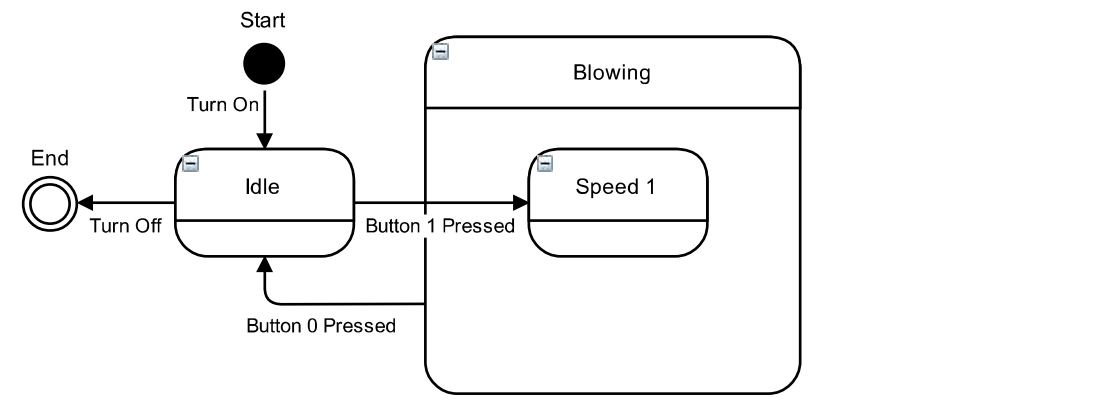
\includegraphics[width=\linewidth]{example-01c}
    \label{example-01c}}
	\caption{The One-Speed Fan example.}
    \label{example-01}
\end{figure}

\subsubsection{Two-Speed Fan Activity}
The Two-Speed Fan activity (Fig. \ref{example-02}) consumes the model that has been produced in the first activity (Model B in Fig. \ref{eoml}). Therefore, any model produced in the previous activity will become the base model for modelling in this activity. Inline to the Flow concept \cite{csikszentmihalyi2014toward}, this second activity has to be more challenging. Therefore, the activity (Fig. \ref{example-02}) challenge learners with one additional state and three new transitions. Now the case has changed. The fan has an additional button, Button 2, to support 2-speed blowing. When Button 1 is pressed, the fan blows in speed 1. When Button 2 is pressed, the fan blows in speed 2. Thus, Learners are required modify the Blowing state into a composite state so it has two speed states. The fan can move from the Idle state to the Speed 1 state, from the Idle state to the Speed 2 state, and from the Speed 1 state to the Speed 2 state or \textit{vice versa}.

\begin{figure}[th]
    \centering
    \subfloat[Base model]{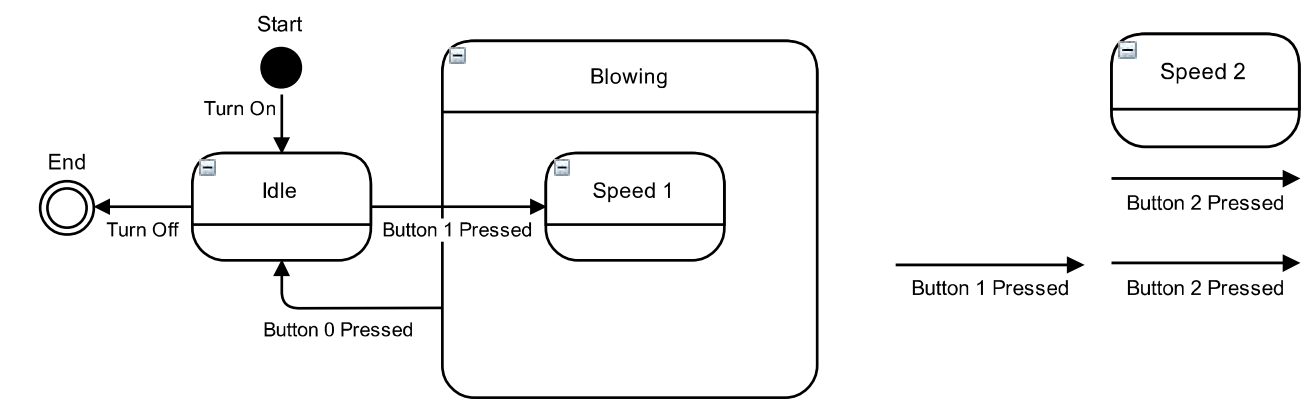
\includegraphics[width=\linewidth]{example-02b}	
    \label{example-02b}}
    \\
    \subfloat[Target model]{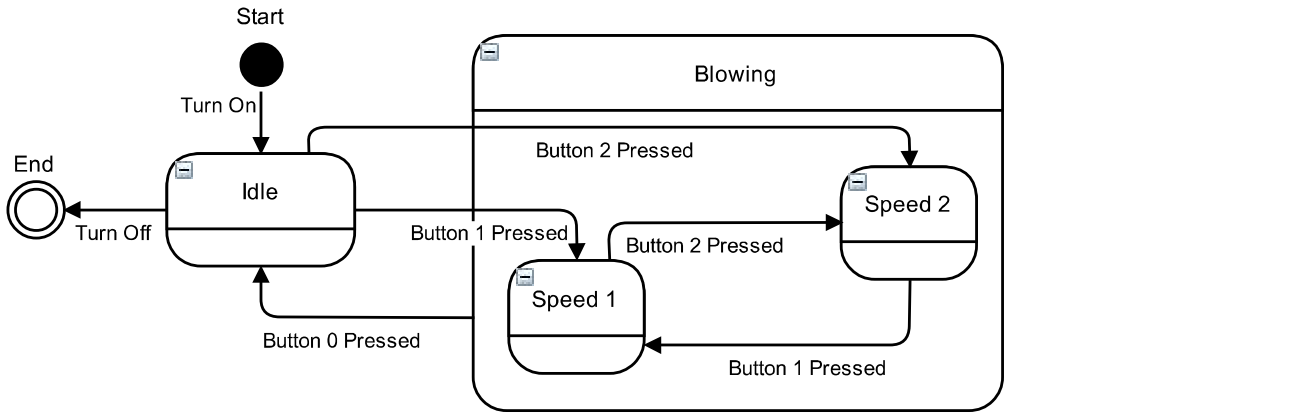
\includegraphics[width=\linewidth]{example-02c}
    \label{example-02c}}
	\caption{The Two-Speed Fan example.}
    \label{example-02}
\end{figure}

\subsubsection{Three-Speed Fan Activity}
The Three-Speed Fan activity (Fig. \ref{example-03}) should be more difficult than the second activity. The fan now supports 3 speeds of blowing, but it has been modified so it cannot go directly to Speed 2 and Speed 3 without firstly go the state with lower speed. In other words, transition from Idle can only go to Speed 1 for the fan to start blowing--Speed 2 and Speed 3 will not be working if transition comes from Idle state. Thus, starting from the model C as the base model as shown in Fig. \ref{eoml}, learners are required to modify the Blowing state into a composite state so it has 3 speeds of blowing and only allow transition from Idle to Speed 1 and from a speed that is lower from the intended one in order to blow.

\begin{figure}[th]
    \centering
    \subfloat[Base model]{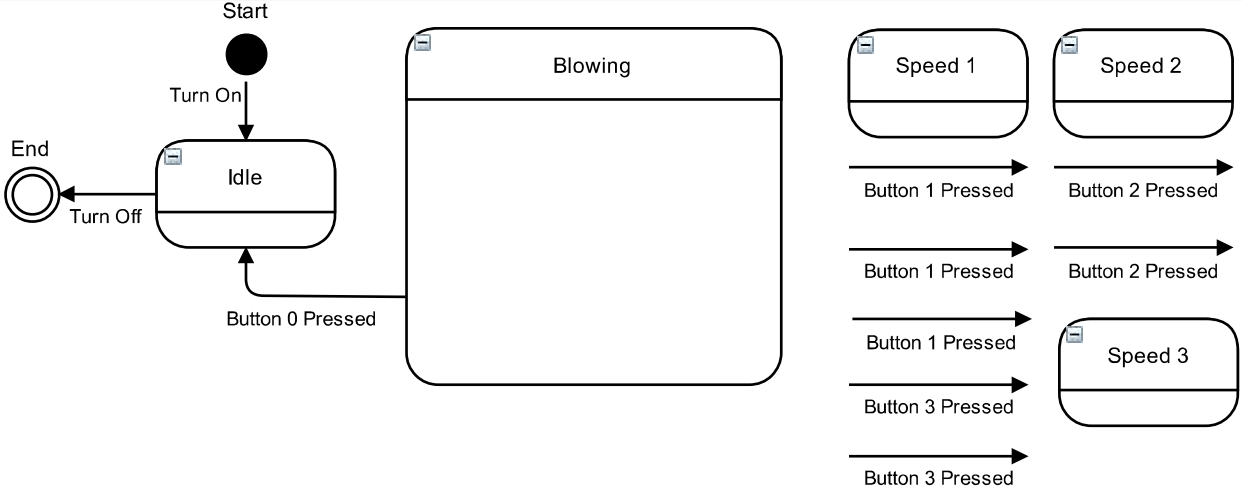
\includegraphics[width=\linewidth]{example-03b}	
    \label{example-03b}}
    \\
    \subfloat[Target model]{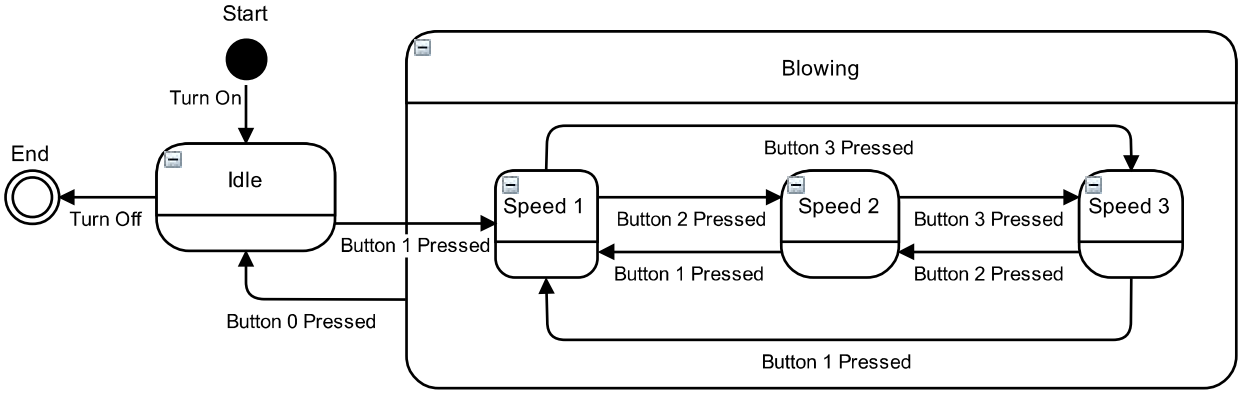
\includegraphics[width=\linewidth]{example-03c}
    \label{example-03c}}
	\caption{The Three-Speed Fan example.}
    \label{example-03}
\end{figure}


\subsection{Generate Game}
After finishing constructing the learning pattern (Fig. \ref{eoml}), designers can now generate a path of levels (or stages) that is usually found in many games. Each generated level corresponds to an activity defined in the learning pattern. The generation also produces an EVL \cite{kolovos2006eclipse} template for each level for its validation to determine whether the level has been completed, all of its objectives have been met, or not. The EVL template is shown in Fig. \ref{validation-template} which can be extended by designers to write code that fits with the level scenarios and objectives. The number of constraints and operations in the template corresponds to the number of objectives defined in the level's learning pattern activity in Fig. \ref{eoml}. As an example implementation of validation, Fig. \ref{validation-realisation} shows the EVL code of checking whether Blowing state has already Speed 1 substate as intended by Objective 1 in One-Speed activity.   

\begin{figure}[th]
\centering
\begin{lstlisting}
context Statechart {
    constraint obj_1 {
        check: 
            self.obj_1()
        message:
            "FAIL: ob_1"
    }
    constraint obj_2 {
        check: 
            self.obj_2()
        message:
            "FAIL: obj_2"
    }        
}
operation Statechart obj_1(): Boolean {
    return true;
}
operation Statechart obj_2(): Boolean {
    return true;
}
\end{lstlisting} 
\caption{Validation template for objectives in One-Speed Fan activity/level.}
\label{validation-template}
\end{figure}

\begin{figure}[th]
\centering
\begin{lstlisting}
context Statechart {
    constraint obj_1 {
        check: 
            self.obj_1()
        message:
            "FAIL: Blowing state contains Speed 1 substate"
    }
    ...
}
operation Statechart obj_1(): Boolean {
    for (state in State.allInstances.select(state | state.name == "Blowing")) {
        if (state.substates.notEmpty() and state.substates.select(substate | substate.name == "Speed 1").notEmpty()){
            return true;
        }        
    }
    return false;
}
...
\end{lstlisting} 
\caption{Validation realisation for Objective 1 in One-Speed Fan activity/level.}
\label{validation-realisation}
\end{figure}

\subsection{Play Game}
After generating the learning pattern into a path of ordered levels and defining its levels' validation, Learners can choose the path and play its levels as depicted in Fig. \ref{path}. When learners choose the first level, an MxGraph-based editor is displayed. Lesson, model description, instruction, objectives, and base model are presented to learners. Learners then can start to modify the base model to reach the target model. 

\begin{figure}[th]
\centering
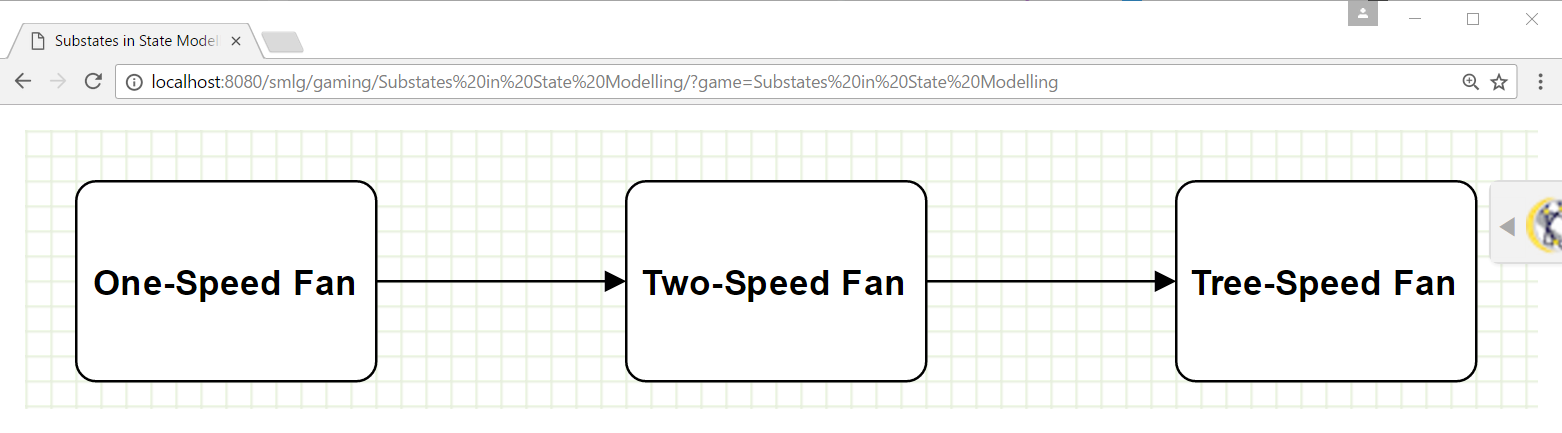
\includegraphics[width=\linewidth]{path}
\caption{The path for learning substate concept with its levels.}
\label{path}
\end{figure}    

Every attempt to change the model will trigger an operation to validate the current model using the defined EVL constraints to assess whether the current model has met the current level's objectives. If not, error messages are displayed to learners indicating the objectives that have not been satisfied. For example, in Fig. \ref{example-fail-messages}, the Speed 1 substate has not been put into the Blowing state even though the Button 1 Pressed transition has connected the Idle state to the Speed 1 substate. If all objectives have been fulfilled, learners have completed the level. A message that congratulate the learners is displayed to give positive reinforcement. Learners then are brought back to the learning path where they can choose the next level to play.  

\begin{figure}[th]
\centering
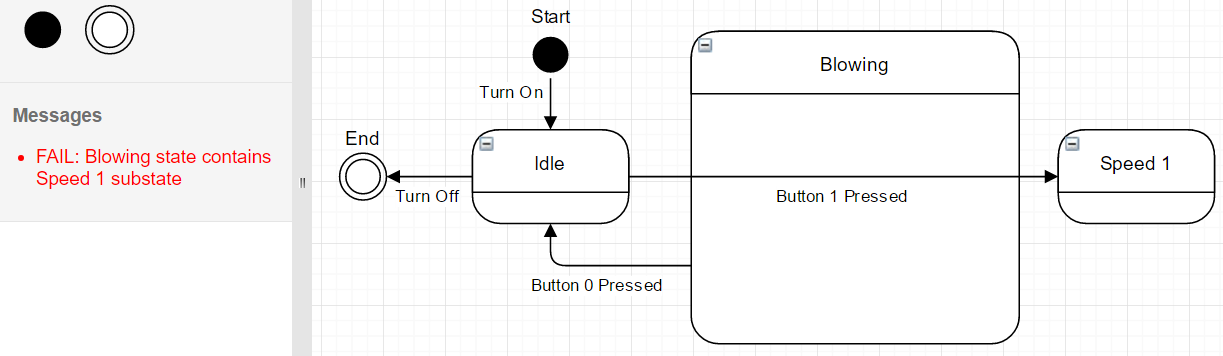
\includegraphics[width=\linewidth]{example-fail-messages}
\caption{A message is displayed to learners indicating the objective that has not been fulfilled.}
\label{example-fail-messages}
\end{figure}  

\section{Challenges and Open Issues}

\section{Related Works}

% An example of a floating figure using the graphicx package.
% Note that \label must occur AFTER (or within) \caption.
% For figures, \caption should occur after the \includegraphics.
% Note that IEEEtran v1.7 and later has special internal code that
% is designed to preserve the operation of \label within \caption
% even when the captionsoff option is in effect. However, because
% of issues like this, it may be the safest practice to put all your
% \label just after \caption rather than within \caption{}.
%
% Reminder: the "draftcls" or "draftclsnofoot", not "draft", class
% option should be used if it is desired that the figures are to be
% displayed while in draft mode.
%
%\begin{figure}[!t]
%\centering
%\includegraphics[width=2.5in]{myfigure}
% where an .eps filename suffix will be assumed under latex, 
% and a .pdf suffix will be assumed for pdflatex; or what has been declared
% via \DeclareGraphicsExtensions.
%\caption{Simulation results for the network.}
%\label{fig_sim}
%\end{figure}

% Note that the IEEE typically puts floats only at the top, even when this
% results in a large percentage of a column being occupied by floats.


% An example of a double column floating figure using two subfigures.
% (The subfig.sty package must be loaded for this to work.)
% The subfigure \label commands are set within each subfloat command,
% and the \label for the overall figure must come after \caption.
% \hfil is used as a separator to get equal spacing.
% Watch out that the combined width of all the subfigures on a 
% line do not exceed the text width or a line break will occur.
%
%\begin{figure*}[!t]
%\centering
%\subfloat[Case I]{\includegraphics[width=2.5in]{box}%
%\label{fig_first_case}}
%\hfil
%\subfloat[Case II]{\includegraphics[width=2.5in]{box}%
%\label{fig_second_case}}
%\caption{Simulation results for the network.}
%\label{fig_sim}
%\end{figure*}
%
% Note that often IEEE papers with subfigures do not employ subfigure
% captions (using the optional argument to \subfloat[]), but instead will
% reference/describe all of them (a), (b), etc., within the main caption.
% Be aware that for subfig.sty to generate the (a), (b), etc., subfigure
% labels, the optional argument to \subfloat must be present. If a
% subcaption is not desired, just leave its contents blank,
% e.g., \subfloat[].


% An example of a floating table. Note that, for IEEE style tables, the
% \caption command should come BEFORE the table and, given that table
% captions serve much like titles, are usually capitalized except for words
% such as a, an, and, as, at, but, by, for, in, nor, of, on, or, the, to
% and up, which are usually not capitalized unless they are the first or
% last word of the caption. Table text will default to \footnotesize as
% the IEEE normally uses this smaller font for tables.
% The \label must come after \caption as always.
%
%\begin{table}[!t]
%% increase table row spacing, adjust to taste
%\renewcommand{\arraystretch}{1.3}
% if using array.sty, it might be a good idea to tweak the value of
% \extrarowheight as needed to properly center the text within the cells
%\caption{An Example of a Table}
%\label{table_example}
%\centering
%% Some packages, such as MDW tools, offer better commands for making tables
%% than the plain LaTeX2e tabular which is used here.
%\begin{tabular}{|c||c|}
%\hline
%One & Two\\
%\hline
%Three & Four\\
%\hline
%\end{tabular}
%\end{table}


% Note that the IEEE does not put floats in the very first column
% - or typically anywhere on the first page for that matter. Also,
% in-text middle ("here") positioning is typically not used, but it
% is allowed and encouraged for Computer Society conferences (but
% not Computer Society journals). Most IEEE journals/conferences use
% top floats exclusively. 
% Note that, LaTeX2e, unlike IEEE journals/conferences, places
% footnotes above bottom floats. This can be corrected via the
% \fnbelowfloat command of the stfloats package.



% conference papers do not normally have an appendix


% use section* for acknowledgment
\section*{Acknowledgment}
This research is part of a doctoral programme supported by \emph{Lembaga Pengelola Dana Pendidikan Indonesia} (Indonesia Endowment Fund for Education).

% trigger a \newpage just before the given reference
% number - used to balance the columns on the last page
% adjust value as needed - may need to be readjusted if
% the document is modified later
%\IEEEtriggeratref{8}
% The "triggered" command can be changed if desired:
%\IEEEtriggercmd{\enlargethispage{-5in}}

% references section

% can use a bibliography generated by BibTeX as a .bbl file
% BibTeX documentation can be easily obtained at:
% http://mirror.ctan.org/biblio/bibtex/contrib/doc/
% The IEEEtran BibTeX style support page is at:
% http://www.michaelshell.org/tex/ieeetran/bibtex/
%\bibliographystyle{IEEEtran}
% argument is your BibTeX string definitions and bibliography database(s)
%\bibliography{IEEEabrv,../bib/paper}
%
% <OR> manually copy in the resultant .bbl file
% set second argument of \begin to the number of references
% (used to reserve space for the reference number labels box)
%\begin{thebibliography}{1}
%
%\bibitem{IEEEhowto:kopka}
%H.~Kopka and P.~W. Daly, \emph{A Guide to \LaTeX}, 3rd~ed.\hskip 1em plus
%  0.5em minus 0.4em\relax Harlow, England: Addison-Wesley, 1999.
%
%\end{thebibliography}

\bibliographystyle{IEEEtran}
\bibliography{references}



% that's all folks
\end{document}


